%%%%%%%%%%%%%%%%%%%%%%%%%%%%%%%%%%%%%%%%%
% Jacobs Landscape Poster
% LaTeX Template
% Version 1.1 (14/06/14)
%
% Created by:
% Computational Physics and Biophysics Group, Jacobs University
% https://teamwork.jacobs-university.de:8443/confluence/display/CoPandBiG/LaTeX+Poster
% 
% Further modified by:
% Nathaniel Johnston (nathaniel@njohnston.ca)
%
% This template has been downloaded from:
% http://www.LaTeXTemplates.com
%
% License:
% CC BY-NC-SA 3.0 (http://creativecommons.org/licenses/by-nc-sa/3.0/)
%
%%%%%%%%%%%%%%%%%%%%%%%%%%%%%%%%%%%%%%%%%

%----------------------------------------------------------------------------------------
%	PACKAGES AND OTHER DOCUMENT CONFIGURATIONS
%----------------------------------------------------------------------------------------

\documentclass[final]{beamer}

\usepackage[scale=1.24]{beamerposter} % Use the beamerposter package for laying out the poster

\usetheme{confposter} % Use the confposter theme supplied with this template

% \setbeamercolor{block title}{fg=ngreen,bg=white} % Colors of the block titles
% \setbeamercolor{block body}{fg=black,bg=white} % Colors of the body of blocks
% \setbeamercolor{block alerted title}{fg=white,bg=dblue!70} % Colors of the highlighted block titles
% \setbeamercolor{block alerted body}{fg=black,bg=dblue!10} % Colors of the body of highlighted blocks
% Many more colors are available for use in beamerthemeconfposter.sty

%-----------------------------------------------------------
% Define the column widths and overall poster size
% To set effective sepwid, onecolwid and twocolwid values, first choose how many columns you want and how much separation you want between columns
% In this template, the separation width chosen is 0.024 of the paper width and a 4-column layout
% onecolwid should therefore be (1-(# of columns+1)*sepwid)/# of columns e.g. (1-(4+1)*0.024)/4 = 0.22
% Set twocolwid to be (2*onecolwid)+sepwid = 0.464
% Set threecolwid to be (3*onecolwid)+2*sepwid = 0.708

\newlength{\sepwid}
\newlength{\onecolwid}
\newlength{\twocolwid}
\newlength{\threecolwid}
\setlength{\paperwidth}{46.8in} % A0 width: 46.8in
\setlength{\paperheight}{33.1in} % A0 height: 33.1in
\setlength{\sepwid}{0.03\paperwidth} % Separation width (white space) between columns
\setlength{\onecolwid}{0.293\paperwidth} % Width of one column
\setlength{\twocolwid}{0.6\paperwidth} % Width of two columns
\setlength{\topmargin}{-0.3in} % Reduce the top margin size
%-----------------------------------------------------------

\newcommand{\vtopsep}[0]{\vspace{0.2ex}}

\usepackage{graphicx}  % Required for including images

\usepackage{booktabs} % Top and bottom rules for tables

\usepackage[hang]{footmisc}

\usepackage{amssymb}

\usepackage{tikz}
\newcommand*\circled[1]{\tikz[baseline=(char.base)]{
			\node[shape=circle,draw,inner sep=2pt] (char) {#1};}}
			
%----------------------------------------------------------------------------------------
%	TITLE SECTION 
%----------------------------------------------------------------------------------------

\title{Protecting Users' Sensitive Data From a Third-Party CDN} % Poster title

\author{Shihan Lin and Xiaowei Yang \\ shihan.lin@duke.edu, xwy@cs.duke.edu} % Author(s)

\institute{\Large{Department of Computer Science, Duke University}} % Institution(s)

%----------------------------------------------------------------------------------------
\renewcommand{\thefootnote}{\fnsymbol{footnote}} 

% \usepackage{enumitem}


\begin{document}

\addtobeamertemplate{block end}{}{\vspace*{2ex}} % White space under blocks
\addtobeamertemplate{block alerted end}{}{\vspace*{2ex}} % White space under highlighted (alert) blocks

\setlength{\belowcaptionskip}{2ex} % White space under figures
\setlength\belowdisplayshortskip{2ex} % White space under equations

\begin{frame}[t] % The whole poster is enclosed in one beamer frame
																										
	\begin{columns}[t] % The whole poster consists of three major columns, the second of which is split into two columns twice - the [t] option aligns each column's content to the top															
		\begin{column}{\sepwid}\end{column} % Empty spacer column
																						        
		\begin{column}{\onecolwid} % The first column                                                  
			\begin{block}{1 Motivation}
				A website which employs a third-party Content Delivery Network (CDN) service faces the following dilemma:
				\vtopsep
				\begin{itemize}
					\item CDN keeps private keys of its customers' certificates so it can observe all traffic between users and its customers.
					\item If clients transfer sensitive data directly to the server, the server's IP address is exposed. It is at the risk of Distributed Denial of Service (DDoS) attacks.
				\end{itemize}
				\vtopsep
				26 of Alexa top 100 sites has purchased third-party CDN service:
				\vtopsep
				\begin{itemize}
					\item 13 sites transfer users' passwords to CDN.
					\item 13 sites expose their IP addresses in the login procedure.
				\end{itemize}
				\vtopsep
				% A protocol providing safety of both users' sensitive data and the server is urgent.
			\end{block}
																																																            
			\begin{block}{2 Related Work}
				\begin{figure}
					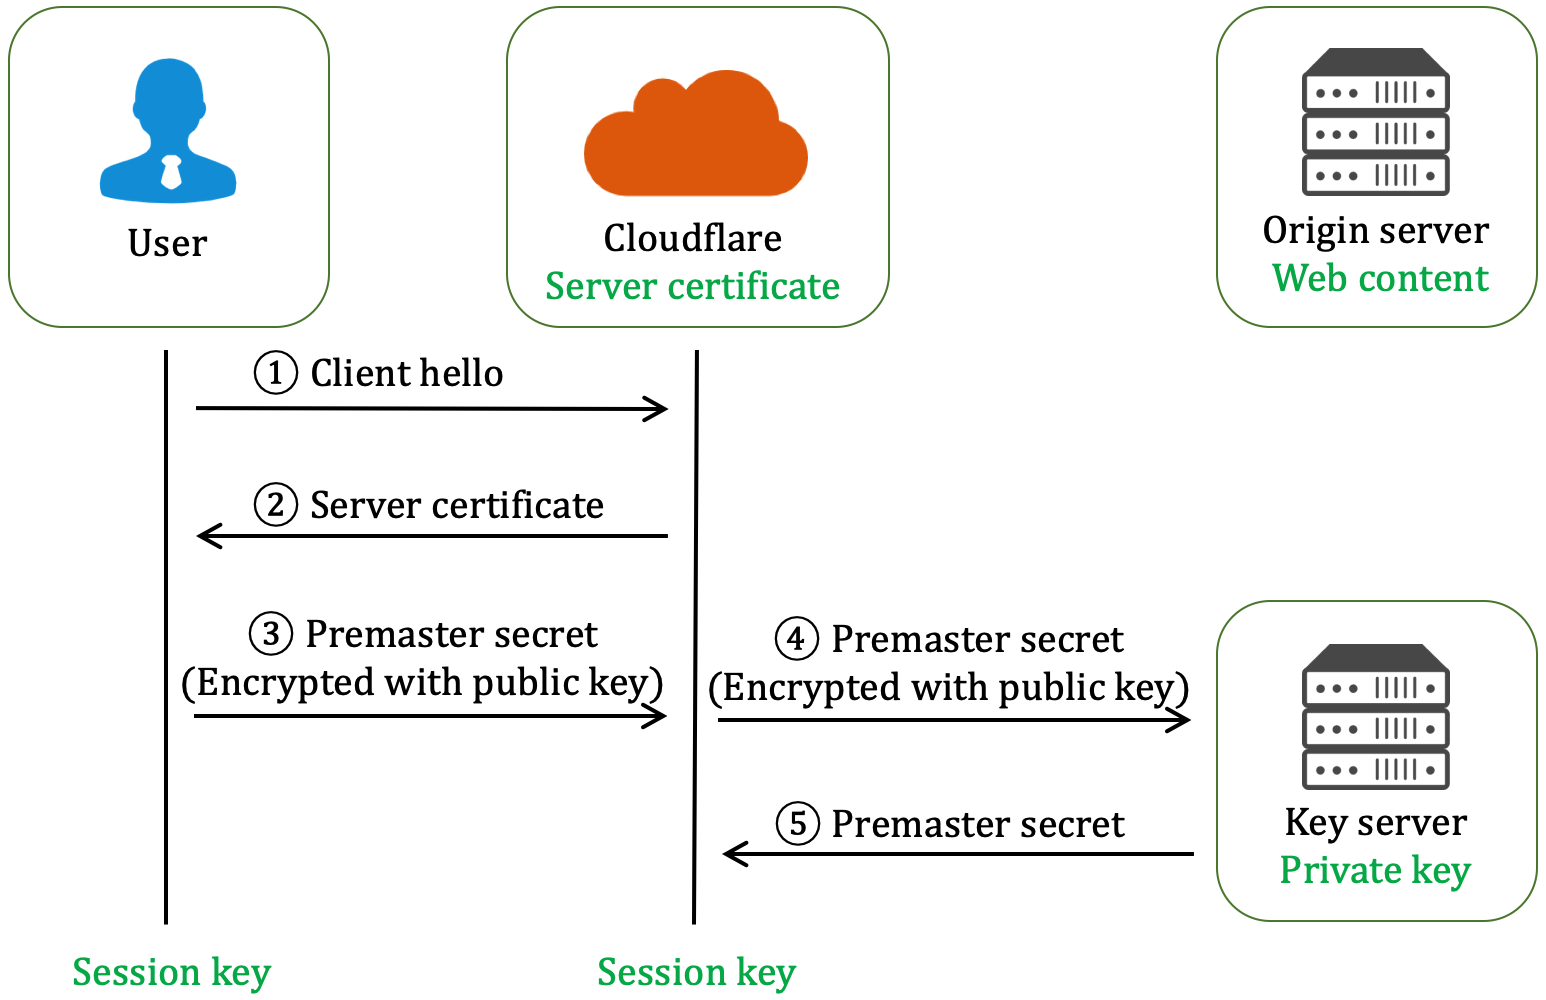
\includegraphics[width=\linewidth]{figures/keyless.png}
					\caption{Cloudflare Keyless SSL proposed in 2014}
				\end{figure}
				\begin{itemize}
					\item Session keys of SSL/TLS are still exposed to CDN.
					\item An open problem proposed in 2016\footnotemark[1]: Eliminating CDNs' need to have session keys.
				\end{itemize}
			\end{block}
																					        
			\footnotetext{*Cangialosi F., etc., Measurement and Analysis of Private Key Sharing in the HTTPS Ecosystem. CCS'16}
																					 
		\end{column} % End of the first column																    
		\begin{column}{\sepwid}\end{column} % Empty spacer column
																																				        
		\begin{column}{\onecolwid} % The second column
			\begin{block}{3 Design}
				\textit{Goals}
				\vtopsep
				\begin{enumerate}
					\item Protecting users' sensitive data from leakage.
					\item Protecting the server from DDoS attacks.
					\item Easy to deploy. No need to modify CDN service and browser.
					\item Compatible with HTTPS. No need to modify HTTPS.
				\end{enumerate}	
				\vtopsep
				\textit{Main idea}
																												
				Add an additional layer of encryption to the client's request over HTTPS and transmit it to the server via CDN.
				\vtopsep
				\begin{itemize}
					\item CDN cannot decrypt the content. Goal~\circled{1} \checkmark %preventing user data leakage.
					\item The server is kept hidden behind CDN. Goal~\circled{2} \checkmark
				\end{itemize}
				\begin{figure}
					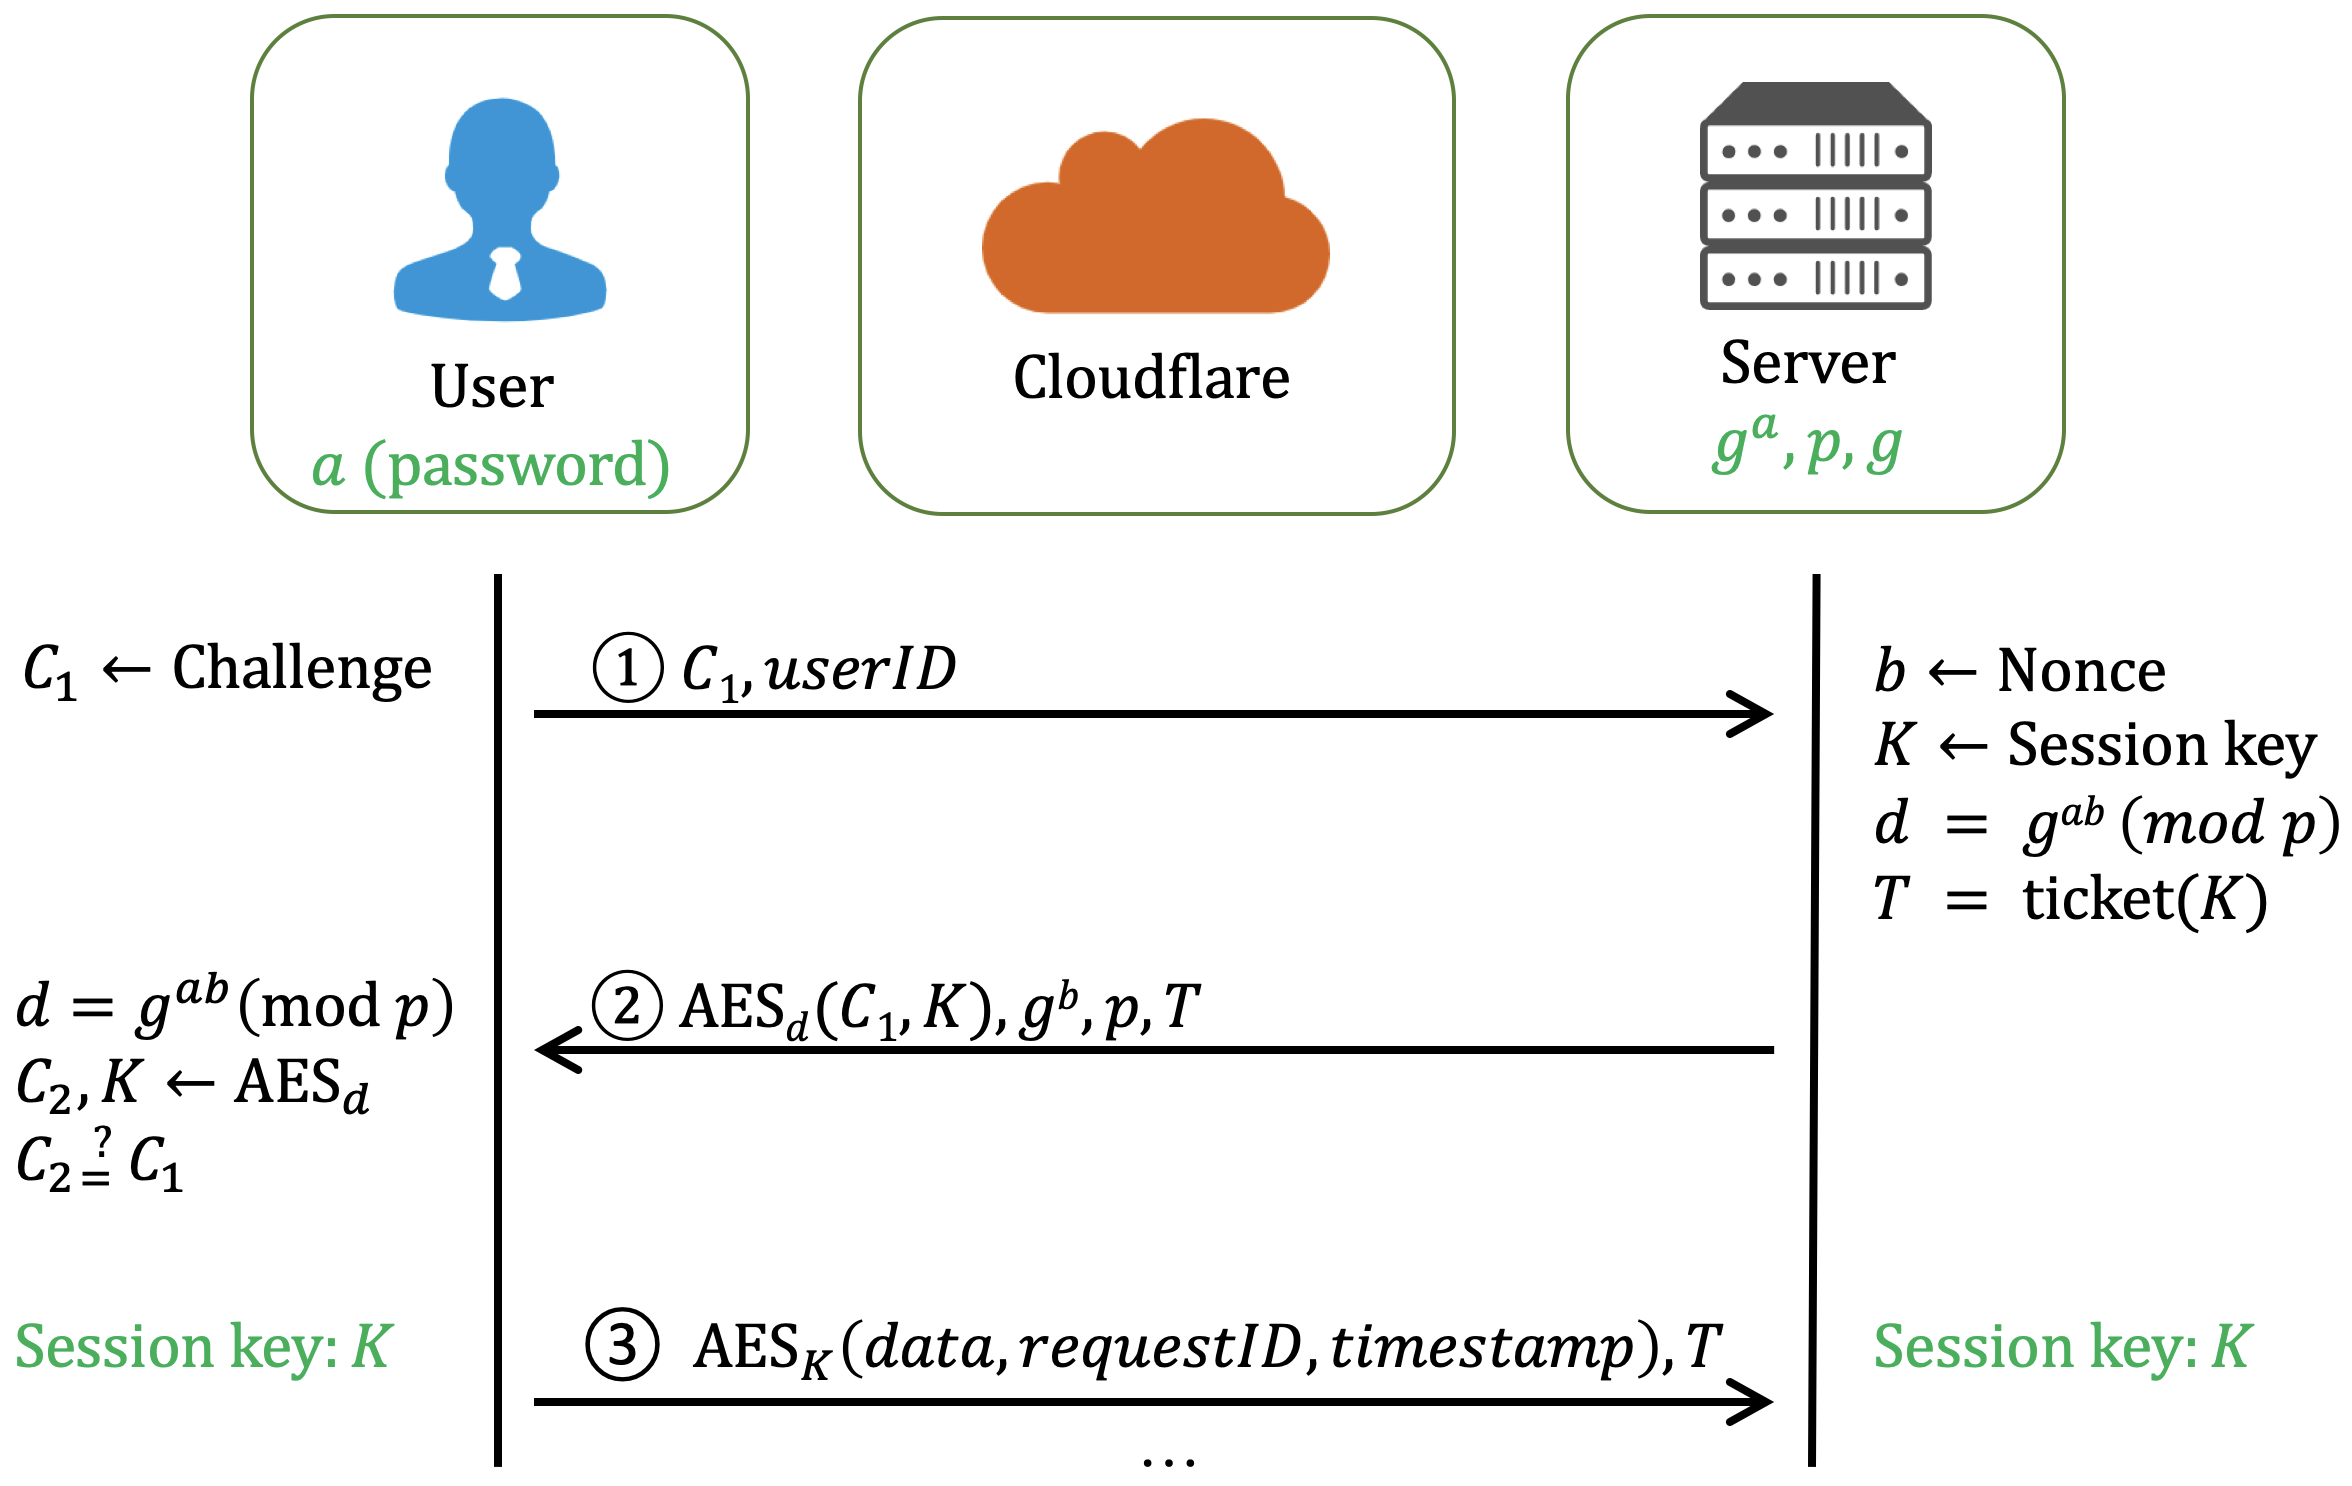
\includegraphics[width=\linewidth]{figures/solution.png}
					\caption{Protocol Design}
				\end{figure}
				\begin{alertblock}{Key Observation}
					The client and server have already shared a common secret, i.e., the user's password.
				\end{alertblock}
				Cloudflare Keyless SSL is employed to remove CDN's access to the private key. The user's password is used as $a$ in Diffie-Hellman algorithm and the server keeps $g^a, g, p$.
			\end{block}
		\end{column} % End of the second column
																																		        
		\begin{column}{\sepwid}\end{column} % Empty spacer column
												
		\begin{column}{\onecolwid} % The third column
			\\
			\rmfamily
			\begin{enumerate}
				\item Client initiates the client hello request with a random challenge number $C_1$ and user ID.
				\item Server retrieves $g^a$ by user ID and generates a nonce $b$ to calculate $g^{ab}$. Server generates the session key $K$ and the TLS session ticket $T$. $C_1$ and $K$ are encrypted by $g^{ab}$ and returned to the client with $g^b, p$ and $T$.
				\item With the password $a$, client calculates $g^{ab}$ and obtains the session key $K$, which is used for future communication.
			\end{enumerate}
			The protocol runs over stateless HTTPS, so the TLS session ticket is required by the server to decrypt messages across HTTPS connections during the session.
			\vspace{3ex}
																		
			\begin{block}{4 Analysis}
				\textit{Security}
				\vtopsep
				\begin{itemize}
					\item User authentication: Only the user knows $a$.
					\item Server authentication: Only the server knows $g^a$, preventing the man-in-the-middle attack
					\item Prevent replay attacks by timestamp and request ID.
					\item Forward security even $g^a$ is leaked. 
					\item CDN plays as a shield against DDoS attacks.
				\end{itemize}
				\vtopsep
				\textit{Implementation and deployment}
				\vtopsep
				\begin{itemize}
					\item Keyless SSL has been deployed on CDN. Goal~\circled{3} \checkmark 
					\item Totally JavaScript implementable. Goal~\circled{3} \checkmark
					\item Run over HTTPS. Goal~\circled{4} \checkmark
					\item Websites' front-end modification is required.
				\end{itemize}
				\vtopsep
			\end{block}
																		
			\begin{block}{5 Limitation}
				\begin{itemize}
					\item Rely on a trust-on-first-use (TOFU) mechanism: Account registration should be secure.
					\item More computation for each communication with sensitive data.
					      % \item Code injection attack: A malicious CDN may inject JavaScript code into HTML of login pages to steal the password.
				\end{itemize}
			\end{block}
			\vspace{-0.5in}
			\begin{figure}
				
\includegraphics[width=0.5\linewidth]{figures/Duke-long.png}
			\end{figure}
		\end{column} % End of the third column
														        
		\begin{column}{\sepwid}\end{column} % Empty spacer column
																
	\end{columns}
																				
\end{frame} % End of the enclosing frame

\end{document}
